\section{Observer agreement}\label{sec:twoway-agree}
Inter-observer agreement is often used as a method of assessing the
reliability of a subjective classification or assessment procedure.
For example, two (or more) clinical psychologists might classify
patients on a scale with categories: normal, mildly impaired,
severely impaired, or ethologists might classify the behavior
of animals in categories of cooperation, dominance and so forth.

A contingency table is formed where the observations are all the
individuals who have been rated or classified.  The rows of the table
refer to the categories used by one observer, while the columns
refer to the categories used by another observer.
In most cases, the same categories are used by both raters,
so the \ctab{} is square, and the entries in the diagonal cells
are the cases where the raters agree.

\begin{Example}[sexisfun1]{Sex is fun} \tabref{tab:sexisfun}
(\citet[Table 2.10]{Agresti:90}, from \citet{Hout-etal:87})
 summarizes the responses of 91
married couples to a questionnaire item:
\begin{quote}
Sex is fun for me and my partner: (a) Never or occasionally, (b)
fairly often, (c) very often, (d) almost always.
\end{quote}
In each row the diagonal entry is not always the largest, though it
appears that the partners tend to agree more often when either responds
``almost always''.
\begin{table}[htb]
\caption[Ratings of a questionnaire item, ``Sex is fun'', by husbands and wives]{Ratings of a questionnaire item, ``Sex is fun'', by husbands and wives. Source: \citet[Table 2.10]{Agresti:90}, from Hout \etal.}\label{tab:sexisfun}
\begin{center}
 \begin{tabular}{l|rrrr|r}
  \hline
            & \multicolumn{4}{c|}{Wife's Rating} & \\
  Husband's & Never & Fairly & Very & Almost &  \\ 
  Rating & fun & often & Often & always & Total \\ 
  \hline
  Never fun     & 7 & 7 & 2 & 3 & 19 \\ 
  Fairly often  & 2 & 8 & 3 & 7 & 20 \\ 
  Very often    & 1 & 5 & 4 & 9 & 19 \\ 
  Almost always & 2 & 8 & 9 & 14 & 33 \\ 
  \hline
  Total & 12 & 28 & 18 & 33 & 91 \\ 
  \hline
 \end{tabular}
\end{center}
\end{table}

\end{Example}

\begin{Example}[MS1]{Diagnosis of MS patients}
\citet{LandisKoch:77} gave data on the diagnostic classification
of multiple sclerosis (MS) patients by two neurologists,
one from Winnipeg and one from New Orleans, who each classified
patients from Winnipeg and New Orleans into one of four
categories:
\begin{seriate}
\item Certain MS,
\item Probable MS,
\item Possible MS,
\item Doubtful, unlikely, or definitely not MS
\end{seriate}
The data from the 69 patients in the New Orleans sample are shown in
\tabref{tab:msdiag}.
There appears to be highest agreement in the Doubtful category, followed by
the Probable category.
\begin{table}[htb]
\caption{Ratings of 69 patients by two neurologists}\label{tab:msdiag}
\begin{center}
 \begin{tabular}{l|rrrr|r}
  \hline
  New Orleans & \multicolumn{4}{c|}{Winnipeg Neurologist} & \\
  Neurologist & Certain & Probable & Possible & Doubtful & Total \\ 
  \hline
  Certain  MS & 5 & 3 & 0 & 0 & 8 \\ 
  Probable MS & 3 & 11 & 4 & 0 & 18 \\ 
  Possible MS & 2 & 13 & 3 & 4 & 22 \\ 
  Doubtful MS & 1 & 2 & 4 & 14 & 21 \\ 
  \hline
  Total       & 11 & 29 & 11 & 18 & 69 \\ 
  \hline
 \end{tabular}
\end{center}
\end{table}


\end{Example}

\subsection{Measuring agreement}\label{sec:agreemeas}
In assessing the strength of agreement we usually have a more
stringent criterion than in measuring the strength of association,
because
observers ratings can be strongly associated without strong agreement.
For example, one rater could use a more stringent criterion and thus consistently rate subjects one category lower (on an ordinal scale) then another rater.
More generally, measures of agreement must take account of the
marginal frequencies with which two raters use the categories.
If observers tend to use the categories
       with different frequency, this will affect measures of
       agreement.
\ix{marginal homogeneity}

\subsubsection{Intraclass correlation}
\ix{intraclass correlation}
\ix{agreement!intraclass correlation}
An analysis of variance framework leads to the {\bf intraclass correlation}
as a measure of inter-rater reliability, particularly when there are
more than two raters.
This approach is not covered here, but various applications are described
by \citet{ShroutFleiss:79}.

\subsubsection{Cohen's Kappa}
\ix{agreement!Cohen's $\kappa$}
\ix{Cohen's $\kappa$|(}
A commonly used measure of agreement,
Cohen's kappa (\(\kappa\))
\citep{Cohen:60,Cohen:68} compares the observed agreement to agreement expected by chance if the two observer's
ratings were independent.
If $p_{ij}$ is the probability that a randomly selected subject is
rated in category $i$ by the first observer and in category $j$ by
the other, then the observed agreement is the sum of the diagonal
entries,  \(P_o  = \sum_i p_{ii}\).  If the ratings were independent,
this probability of agreement (by chance) would be \(P_c = \sum_i p_{i+} \,  p_{+i}\).
Cohen's $\kappa$ is then the ratio of the difference between actual
agreement and chance agreement, $P_o - P_c$, to the maximum value
this difference could obtain:

\begin{equation}\label{eq:kappa}
  \kappa =  \frac{ P_o - P_c } { 1 - P_c }
  \period
\end{equation}

When agreement is perfect, \(\kappa = 1\);  when agreement is no
better than would be obtained from statistically independent ratings,
$\kappa = 0$.
$\kappa$ could conceivably be negative, but this rarely occurs in practice.
The minimum possible value depends on the marginal totals.

For large samples ($n_{++}$), $\kappa$ has an approximate normal
distribution when $H_0 : \kappa = 0$ is true
and its standard error \citep{Fleiss:73,Fleiss-etal:69} is given by
\begin{equation*}
 \hat{\sigma}(\kappa) =  \frac{ P_c + P_c^2 - \sum_i p_{i+} p_{+i} (p_{i+} + p_{+i}) } { n_{++} (1 - P_c)^2 }
 \period
\end{equation*}
Hence, it is common to conduct a test of $H_0 : \kappa = 0$ by
referring $z = \kappa / \hat{\sigma}(\kappa)$
to a unit normal distribution.
The hypothesis of agreement no better than chance is rarely of much
interest, however.  It is preferable to estimate and report a
confidence interval for $\kappa$.

\subsubsection{Weighted Kappa}
The original (unweighted) \(\kappa\) only counts strict agreement (the same
 category is assigned by both observers).  A weighted version of
       \(\kappa\)
                 \citep{Cohen:68} may be used when one wishes to allow for partial agreement.
       For example, exact agreements might be given full weight,
       one-category difference given weight 1/2.  This typically makes sense
       only when the categories are ordered, as in severity of
       diagnosis.

Weighted \(\kappa\) uses weights, $0 \le w_{ij} \le 1$ for each cell in the
table, with $w_{ii} =1$ for the diagonal cells.
In this case $P_o$ and $P_c$ are defined as weighted sums
\begin{eqnarray*}
P_o  & = & \sum_i \sum_j w_{ij} p_{ij} \\
P_c  & = & \sum_i \sum_j w_{ij} p_{i+} p_{+j}\\
\end{eqnarray*}
and these weighted sums are used in \eqref{eq:kappa}.

For an $r \times r$ table, two commonly-used pattern of weights are those based on
equal spacing of weights
\citep{CicchettiAllison:71}
for a near-match,
%$w_{ij} = 1 - \frac{|i-j|}{r-1}$
and
\emph{Fleiss-Cohen weights}
\citep{FleissCohen:73}, based on an inverse-square
spacing,
% $w_{ij} = 1 - \frac{|i-j|^2}{(r-1)^2}$.
\begin{eqnarray*}
w_{ij} = & 1 - \frac{|i-j|}{r-1} & \quad\quad\mbox{equal spacing} \\
w_{ij} = & 1 - \frac{|i-j|^2}{(r-1)^2} & \quad\quad\mbox{Fleiss-Cohen}
\end{eqnarray*}
\PROC{FREQ} uses the integer (equal) spacing weights by default.
The Fleiss-Cohen weights attach greater importance
to near disagreements, as you can see below for a $4 \times 4$ table.
These weights also provide a measure equivalent to the intraclass
correlation.

\begin{verbatim}
       Integer Spacing                 Fleiss-Cohen Weights
   1     2/3     1/3       0          1     8/9     5/9      0
 2/3       1     2/3     1/3        8/9       1     8/9    5/9
 1/3     2/3       1     2/3        5/9     8/9       1    8/9
   0     1/3     2/3       1          0     5/9     8/9      1
\end{verbatim}

\subsubsection{Computing Kappa with SAS}
In \sasver{6.10} and later, \PROC{FREQ}
provides the $\kappa$ statistic with the \opt{agree}{FREQ}, as shown in
the following example.%
\footnote{In \sasver{7} \PROC{FREQ}
provides 
the \stmt{TEST}{FREQ}
with syntax \pname{TEST KAPPA;} to test the hypothesis that $\kappa = 0$.
You can also request Fleiss-Cohen weights with the option \pname{AGREE (WT=FC)}
in the \stmt{TABLES}{FREQ}.
Standard errors, confidence intervals, and test statistics are large-sample (asymptotic)
by default.  Exact tests are provided by the \stmt{EXACT AGREE}{FREQ}
in \sasver{7}.}

\begin{listing}
title 'Kappa for Agreement';
data fun;
   label husband = 'Husband rating'
         wife    = 'Wife Rating';
   do husband = 1 to 4;
   do wife    = 1 to 4;
      input count @@;
      output;
      end; end;
datalines;
 7     7     2      3
 2     8     3      7
 1     5     4      9
 2     8     9     14
;
proc freq;
   weight count;
   tables husband * wife / noprint agree;
run;
\end{listing}
\ixd{Sex is fun}

This produces the output shown in \outref{out:sexagree}.
Simple kappa gives the unweighted value; you can see there is little
evidence of agreement beyond chance in husbands' and wives' ratings
of their sexual fun.
Weighted kappa uses the equal spacing weights, taking into account
ratings which `nearly' agree.  The weighted sample $\kappa$ is
larger, and the confidence interval does not include 0,
so the weighted agreement is significantly greater than chance,
though again we see that agreement is relatively small.
The test of symmetry (Bowker's test) shown in \outref{out:sexagree}
tests the null hypothesis that non-agreements are symmetric.
\begin{Output}
\caption{Sex is fun data, agreement analysis}\label{out:sexagree}
\small
\verbatiminput{ch3/out/sexagree.out}
\end{Output}
\ix{Cohen's $\kappa$|)}

\subsection[Observer Agreement Chart]{Bangdiwala's Observer Agreement Chart}
\label{sec:twoway:Bangdiwala}
\ix{agreement!observer agreement chart|(}
\ix{observer agreement chart|(}
The observer agreement chart by
\citet{Bangdiwala:87} provides a simple
graphic representation of the strength of agreement in a contingency
table, and a measure of strength of agreement with an intuitive
interpretation.

The agreement chart is constructed as an \(n \times  n\) square,
where $n$ is the total sample size.  Black squares, each of size
\(n_{ii} \times  n_{ii}\), show observed agreement.  These are positioned
within larger rectangles, each of size \(n_{i+} \times  n_{+i}\)
as shown in \figref{fig:agree11}.  The
large rectangle shows the maximum possible agreement, given the
marginal totals.  Thus, a visual impression of the strength of
agreement is given by
\begin{equation}\label{eq:bangb}
  B_N  =
  \frac{ \mbox{area of dark squares}}
  { \mbox{area of rectangles}}  =
  \frac{ \sum_i^k \,  n_{ii}^2 }
  { \sum_i^k \,  n_{i+} \,  n_{+i} }
\end{equation}

\begin{figure}[htb]
  \centering
  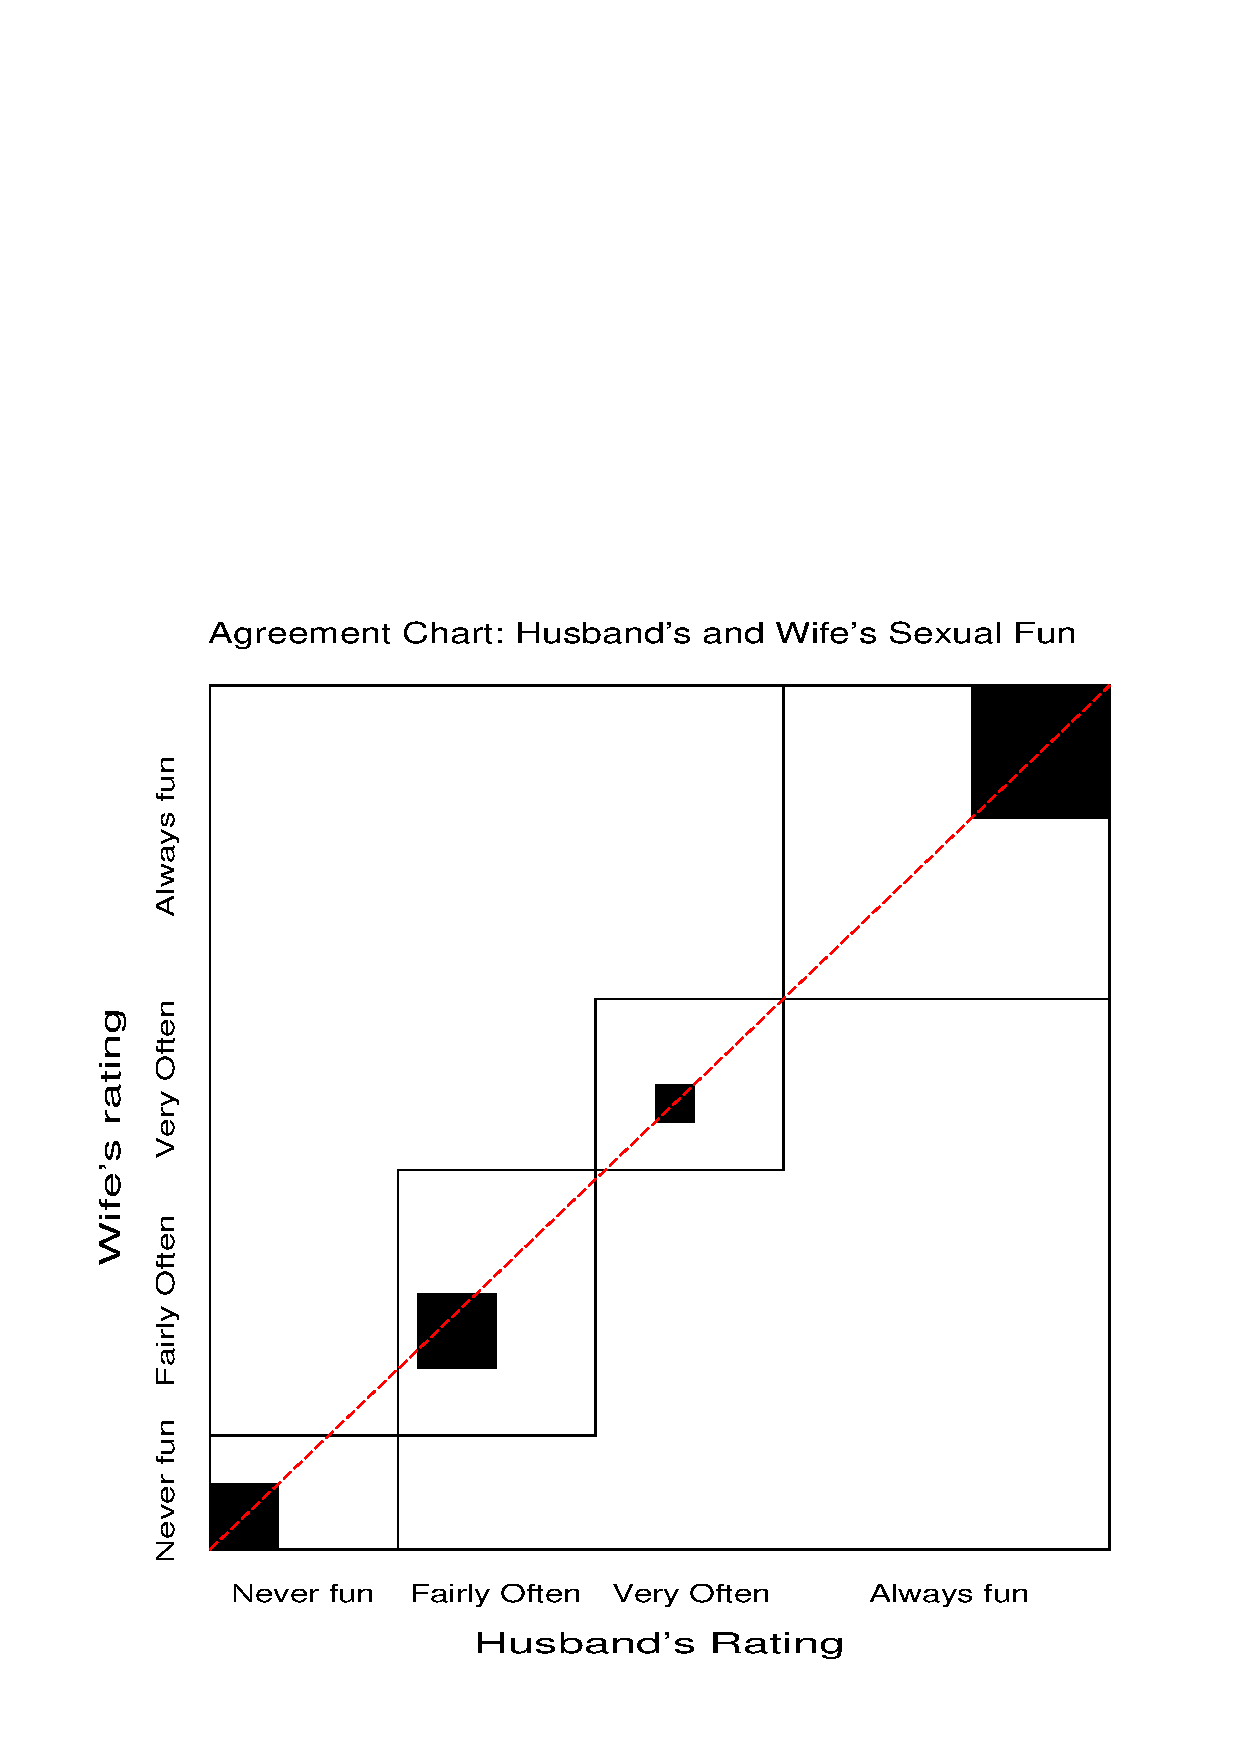
\includegraphics[scale=.5]{ch3/fig/agree11}
  \caption[Agreement chart]{Agreement chart for husbands and wives
sexual fun.  The \(B_N\) measure \eqref{eq:bangb} is the ratio of the areas of the
dark squares to their enclosing rectangles, counting only exact
agreement.  \(B_N = 0.146\) for these data.}\label{fig:agree11}

\end{figure}

\subsubsection{Partial agreement}
\ix{agreement!partial}
 Partial agreement is allowed by
including a weighted contribution from off-diagonal cells, $b$
steps from the main diagonal.  For a given cell frequency,
$n_{ij}$, a pattern of weights, $w_1, w_2, \dots,  w_b$ is applied
to the cell frequencies
as shown schematically below:
\begin{equation*}
 \left.
 \begin{array}{ccccc}
   &  & n_{i-b,i} &  & \\
        &  & \vdots    &  & \\
        n_{i, i-b} & \cdots & n_{i, i} & \cdots & n_{i, i+b} \\
        &  & \vdots    &  & \\
   &  & n_{i-b,i} &  &
 \end{array}
  \right.
  \qquad
 \left.
 \begin{array}{ccccc}
   &  & w_b &  & \\
   &  & \vdots &  & \\
 w_b & \cdots & 1 & \cdots & w_b \\
   &  & \vdots &  & \\
   &  & w_b &  & \\
 \end{array}
  \right.
\end{equation*}

These weights are incorporated in the agreement chart (\figref{fig:agree12}) by successively lighter
shaded rectangles whose size is proportional to the sum of the cell
frequencies, denoted \(A_{bi}\), shown above.  \(A_{1i}\)
allows 1-step disagreements, using weights 1 and $w_1$;
\(A_{2i}\) includes 2-step disagreements,
etc.  From this, one can define a weighted measure of agreement,
analogous to weighted \(\kappa\).
\begin{equation*}
  B_N^w  =
  \frac{ \mbox{weighted sum of areas of agreement}}
  { \mbox{area of rectangles} }  =
  1 - \frac{ \sum_i^k \,
  [ n_{i+} n_{+i} - n_{ii}^2  -
  \sum_{b=1}^q \,  w_b  A_{bi} ] }
  { \sum_i^k \,  n_{i+} \,  n_{+i} }
\end{equation*}
where \(w_b\) is the weight for \(A_{bi}\), the shaded area $b$ steps
away from the main diagonal, and $q$ is the furthest level of partial
disagreement to be considered.

\begin{figure}[htb]
  \centering
  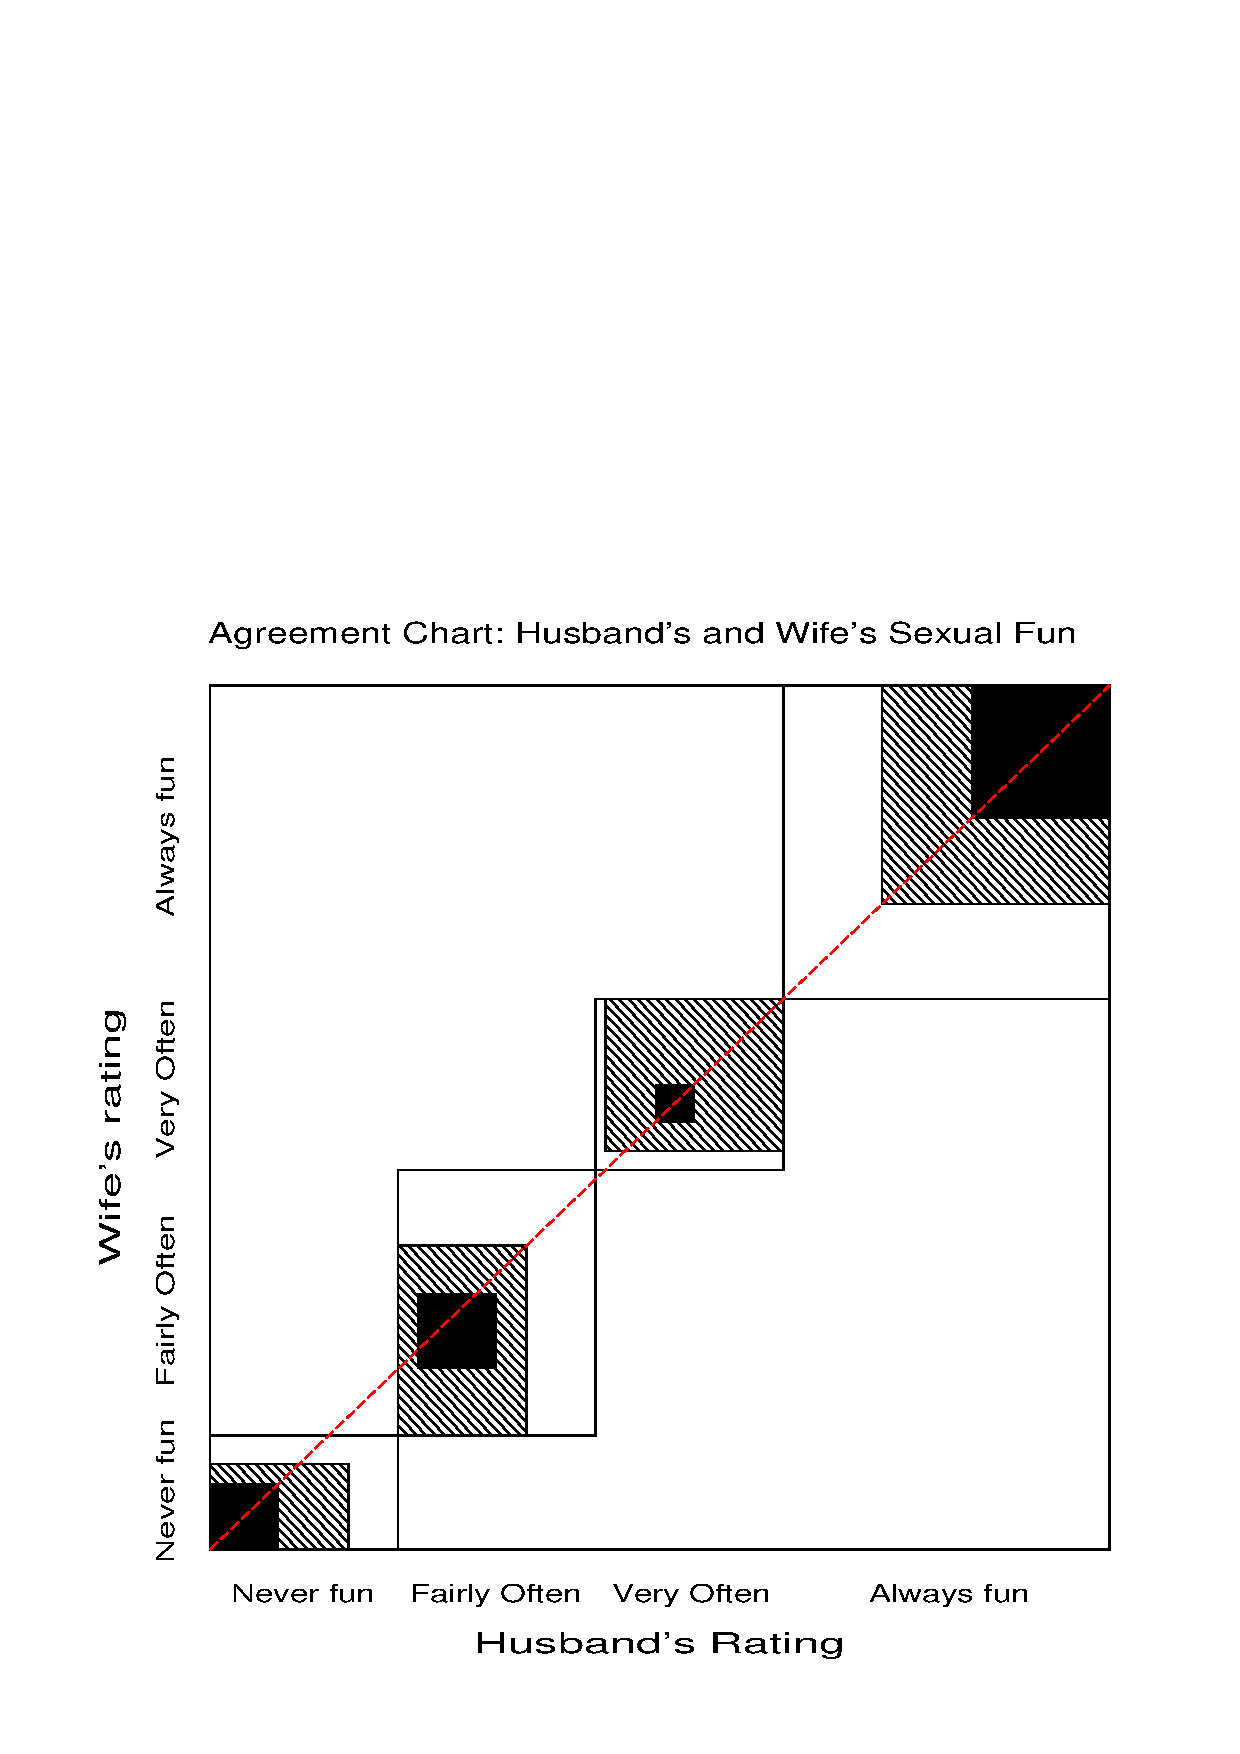
\includegraphics[scale=.5]{ch3/fig/agree12}
  \caption[Weighted agreement chart]{Weighted agreement chart.  The
\(B_N^w\) measure is the ratio of the areas of the dark squares to
their enclosing rectangles, weighting cells one step removed from
exact agreement with \(w_1 = 8 / 9 = .889\).  \(B_N^w  =
0.628\) for these data.}\label{fig:agree12}
\end{figure}

\subsection{Observer bias}\label{sec:Observer}

With an ordered scale, it may happen that one observer consistently
tends to classify the objects into higher or lower categories than
the other.  This produces differences in the marginal totals,
\(n_{i+}\), and \(n_{+i}\).  While special tests exist for
\boldital{marginal homogeneity}, the observer agreement chart shows this
directly by the relation of the dark squares to the diagonal line:
When the marginal totals are the same, the squares fall along the
diagonal.
\ix{marginal homogeneity}

\begin{Example}[MS2]{Diagnosis of MS patients}
\tabref{tab:msdiag} shows the classification of
69 New Orleans patients regarding multiple sclerosis diagnosis by
neurologists in New Orleans and Winnipeg.  The complete \Dset,
listed in \datref{dat:msdiag}, also includes 149 Winnipeg patients who
were assessed by both neurologists.

It is instructive to compare the agreement charts for the two patient
samples, shown in
\figref{fig:agree2}.
For both groups of patients,
the two intermediate categories lie largely above the line,
indicating that the Winnipeg neurologist tends to classify patients
into more severe diagnostic categories.
The departure from the diagonal is greater for the Winnipeg patients,
for whom the Winnipeg neurologist uses the two most severe diagnostic
categories very often.
\ixd{multiple sclerosis diagnosis}

\begin{figure}[htb]
  \centering
  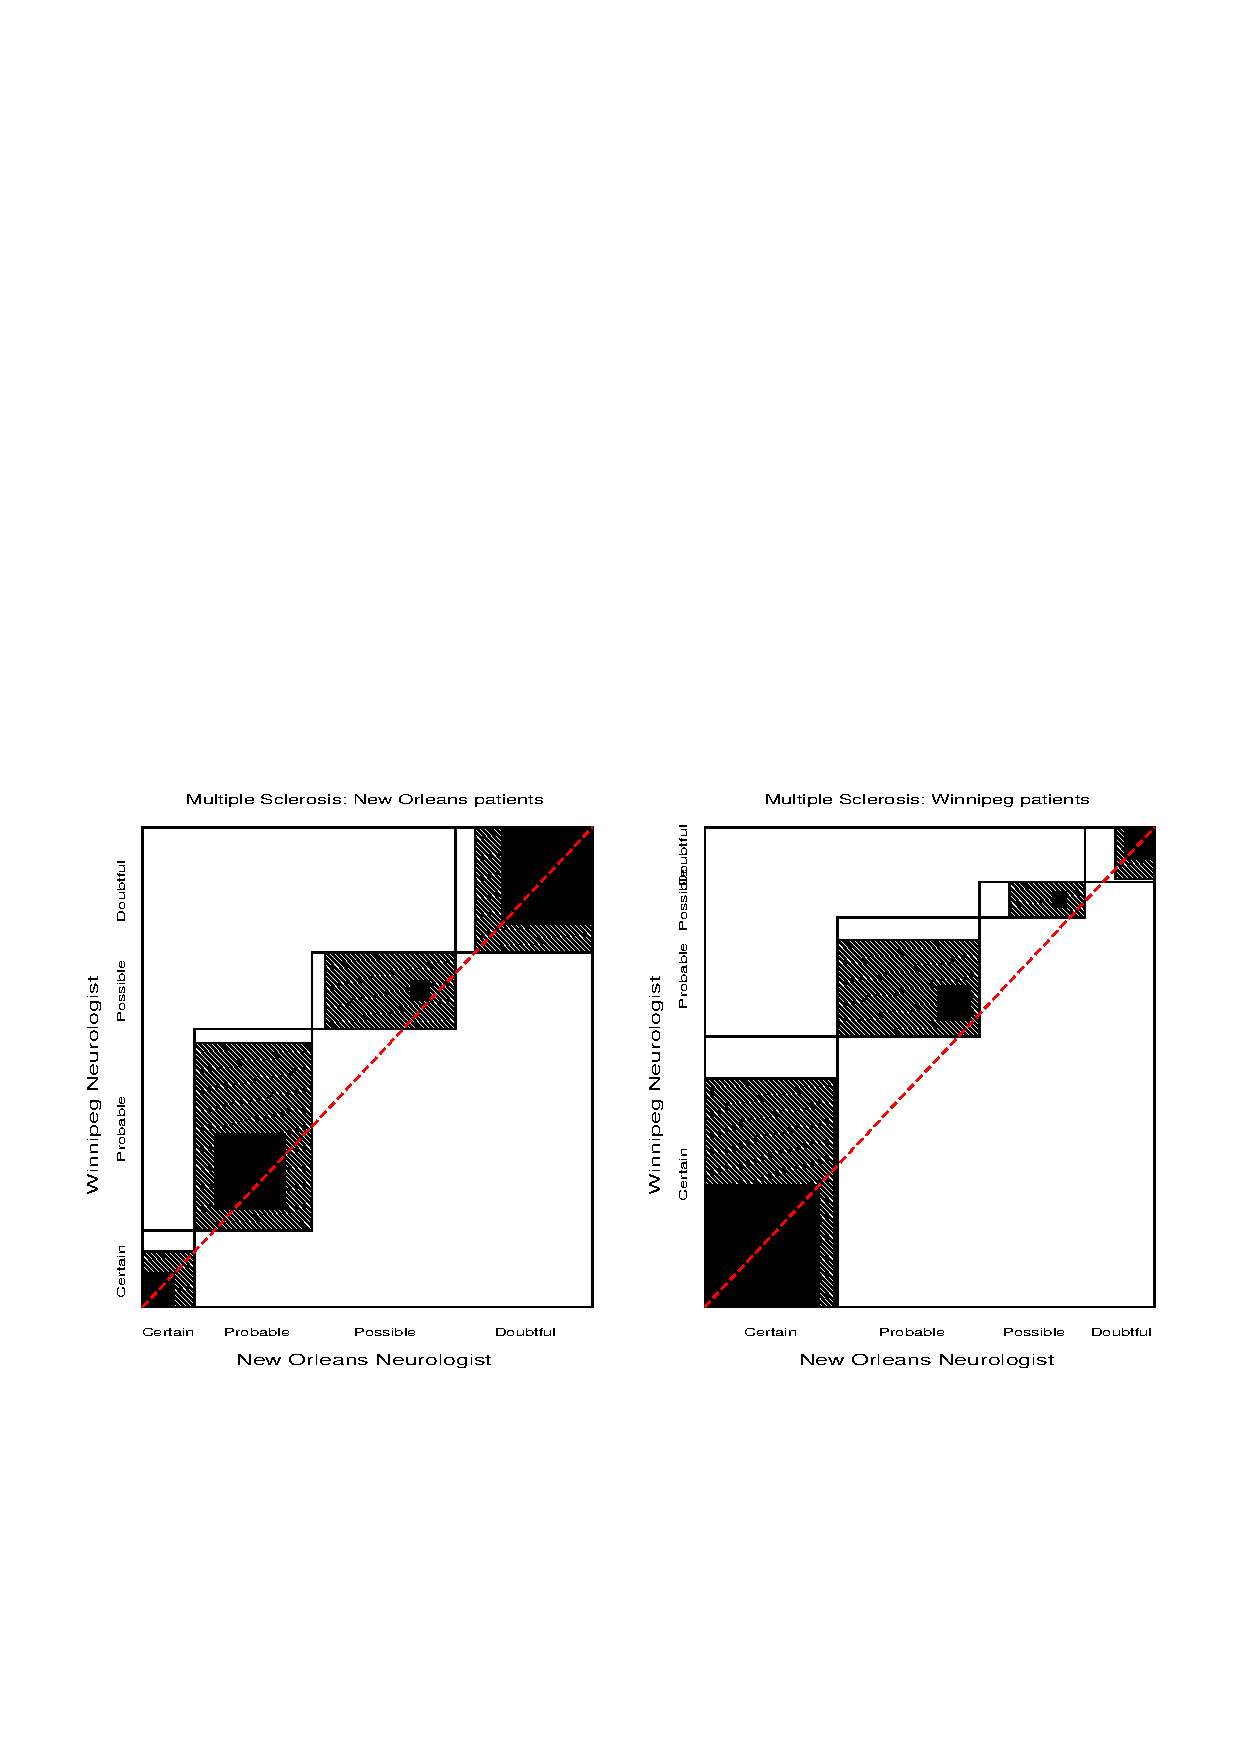
\includegraphics[width=1\linewidth,clip]{ch3/fig/agree2}
  \caption[Weighted agreement chart]{Weighted agreement chart for the MS data.  Departure of the middle squares from the diagonal indicates lack of marginal homogeneity.}\label{fig:agree2}
\end{figure}
\end{Example}

\subsection{The \sasprog{AGREE}}
The observer agreement charts are produced by the \sasprog{AGREE},
which is listed and described in \macref{mac:agree}.
It is written in \IML{} and so is used like the \sasprog{SIEVE}:
\begin{listing}
run agree(table,w, vnames, lnames, title);
\end{listing}

In addition to the \texttt{TABLE}, \texttt{VNAMES}, and \texttt{LNAMES}
arguments,
the \texttt{AGREE} module takes a vector \texttt{W} of one or more weights
to specify the number of steps of disagreement, and the weight to be
applied to each.
The following statements produce \figref{fig:agree11} and
\figref{fig:agree12}.
In the first call to \texttt{AGREE}, \texttt{w=1}, so only exact
agreement is considered; in the second call, \texttt{w=\{1 .889\}},
so 1-step disagreements are given weights of $\frac89$.
%% input: /users/faculty/friendly/sasuser/catdata/agree1.sas
%% last modified: 15-Jan-98 15:25
\begin{listing}
title "Observer Agreement Chart";
proc iml;
   %include agree;
   table =
     \{  7     7     2      3,
        2     8     3      7,
        1     5     4      9,
        2     8     9     14 \};
   title  = "Agreement Chart: Husband's and Wife's Sexual Fun";
   vnames = \{"Husband's Rating" "Wife's rating"\};
   lnames = \{'Never fun' 'Fairly Often' 'Very Often' 'Always fun'\} ;
   font = 'hwpsl009';
   
   w=1;                     /* \figref{fig:agree11} */
   run agree(table, w, vnames, lnames, title);
   w = w || (8/9);          /* \figref{fig:agree12} */
   run agree(table, w, vnames, lnames, title);
   end;
quit;
\end{listing}

\ix{observer agreement chart|)}
\ix{agreement!observer agreement chart|)}
